\section{Tutorial zu Gephi}\label{tutorial}
\subsection*{Erläuterungen der Dateien}
In diesem Teil wird ein Tutorial zu dem Open Source Programm Gephi beschrieben. Diese Program liest hauptsächlich .gexf Dateiformate ein und erstellt dann aus diesen ein Netzwerk aus Knoten und Kanten. gexf Dateien sind in einem speziellen XML Format geschrieben und können sehr viele Informationen und Attribute übergeben. Die Dateien für dieses Tutorial wurden in R mit den Skripten gexf.R und gexf\_support.R erstellt. Mit den Skripten können verschiedene Parameter und Attribute übergeben werden, wie zum Beispiel die farbliche Kodierung der Knoten und die Gewichtung der Kanten. Das Format der bearbeiteten Netzwerke sind .gephi Dateien, die ausschlieslich in Gephi eingelesen werden können. In diesen sind dann typischerweise Layouts und gefilterte Graphen gespeichert. Die nachfolgende Tabelle gibt eine Übersicht über die .gexf und .gephi Dateien, die im elektronischen Anhang bereits vorhanden sind und mit Hilfe deren das Tutorial beschrieben wird.


\begin{table}[H]
    \begin{center}
        \begin{tabular}{|c|p{7cm}|} 
            \hline  relative\_ausgaenge.gexf  & unbearbeiteter Graph, die ersten 100 Position sind als Knoten dargestellt, Gewichtung der Kanten sind die relativen Ausgaenge \\
            \hline  relative\_ausgaenge\_pos\_10.gexf  & unbearbeiteter und gefilteter Graph, die ersten 10 Position sind als Knoten dargestellt , Gewichtung der Kanten sind die relativen Ausgaenge \\
            \hline  relative\_ausgaenge\_pos\_10\_Layout.gephi  & bearbeiteter Graph mit Layout, die ersten 10 Position sind als Knoten dargestellt , Gewichtung der Kanten sind die relativen Ausgaenge und die Knoten sind nach relativen Haeufigkeiten gewichtet\\
            \hline  relative\_gaenge.gexf  & unbearbeiteter Graph, die ersten 100 Position sind als Knoten dargestellt, Gewichtung der Kanten sind die relativen Ausgaenge \\  
            \hline  relative\_eingaenge\_pos\_10.gexf  & unbearbeiteter und gefilteter Graph, die ersten 10 Position sind als Knoten dargestellt , Gewichtung der Kanten sind die relativen Ausgaenge \\
            \hline relative\_eingaenge\_pos\_10\_Layout.gephi  & bearbeiteter Graph mit Layout, die ersten 10 Position sind als Knoten dargestellt , Gewichtung der Kanten sind die relativen Ausgaenge und die Knoten sind nach relativen Haeufigkeiten gewichtet \\     
            \hline
        \end{tabular} 
    \end{center}
    \caption{Übersicht der Gephi Dateien}\label{Gephi_dateien}
\end{table}

\subsection*{Erste Schritte mit Gephi}
Nach der Installation und öffnen des Programs, kann man über $ \rightarrow $ File $ \rightarrow $ Open, die Dateien öffnen und bei dieser Datenlage ist der Import Report zu vernachlässigen. Die folgende Abbildung zeigt den Workspace nach dem Laden der relative\_ausgaenge.gexf Datei. Im lila Kasten sind die einzelnen Bearbeitungsmodi von Gephi. Overview ist dafür gedacht den Graphen zu bearbeiten und mit einem Layout zu versehen. Im Data Labratory kann man einzelne Knoten und Kanten bearbeiten und neue Attribute hinzufügen. Der Preview ist dann eine Vorschau von der Datei die exportiert wird und kann hierzu auch noch weiter verändert werden. Außerdem befindet sich hier der Export der Graphen.Gelb markiert sind die Daten, die als Knoten und Kanten dargestellt sind. Diese quaderförmige Struktur besitzt der Graph nur am Anfang und wird durch den blauen Kasten auf der linken Seite verändert. Hier kann man den gewünschten Algorithmus auswählen, der die Position der Knoten berechnet und durch Parameter eingestellt werden kann. Zum Beispiel haben wir die Parameter \textit{Edge Weight Influence}, dass den Einfluss der Gewichtung der Kanten steuert, auf $ 0.1 $. Das \textit{Scaling} , die Größe des Graphen , wurde auf $ 200 $ festgelegt und \textit{Approximate Repulsion} , zuständig für die Konvergenz des Graphen, wurde nicht makiert damit es einen größeren und übersichtlicheren Graphen ergibt. Am Ende des Algorithmus wurde noch das \textit{Prevent Overlap} aktiviert um keine Überlappungen der Knoten zu haben. \\
Um das Layout und die Struktur weiter zu beeinflußen , kann man in dem linken roten Kasten die Größe der Kanten und der Knoten definieren, dabei muss der rote Diamant ausgewählt werden und ein Gewichtungsattribut ausgewählt werden, in unserem Fall die Variable \textit{relative}, die den relativen Häufigkeiten der auftretenden Knoten in einer Position entspricht. Im grünen Feld daneben befinden sich die Optionen für die Maus, wie zum Beispiel die voreingestellte Fähigkeit, dass man Knoten manuell im Graphen bewegen und positionren kann. Aber auch die letzte Option ist hilfreich, mit der man durch einen Klick auf einen Knoten, dessen beinhaltete Information ersehen kann. Die Boxen auf der linken Seite dienen hauptsächlich dazu den Graphen zu filtern und in einen neuen Workspace zu exportieren.\\
Im linken Roten Feld kann man \textit{Statistics} und \textit{Filters} anwenden, bei den Filtern handelt es sich um die übergebenen Attribute nach denen Gefilter werden kann. Bei \textit{Partition} befindet sich die Position als Attribute, mit der eingestellt werden kann welche Position im Graphen angezeigt werden kann. Diesen Filter muss man dann in den grünen Kasten ziehen um dann die Auswahlmöglichkeiten im blauen Kasten zu bekommen. Hier kann kann man dann die gewünschten Position dann auswählen und mittels dem Button \textit{Filter} aktivieren. Desweiteren kann man auch einen \textit{subfilter}, also einen zweiten Filter gleichzeitig anwenden und hier empfiehlt sich dann das \textit{Edge Weight}. Generell empfiehlt es sich, dass man erst den Graphen nach seinen Interessen filtert und dann den Layout Algorithmus anwendet, da sich dieser je nach Filterung anpasst. Weitere hilfreiche Features des Programs befinden sich in der Fußzeile des Workspaces, wie zum Beispiel das ein- oder ausblenden von Knotenlabels mithilfe des großen \textit{T} oder der Screenshot Funktion.

\begin{figure}[H]
    \centering
    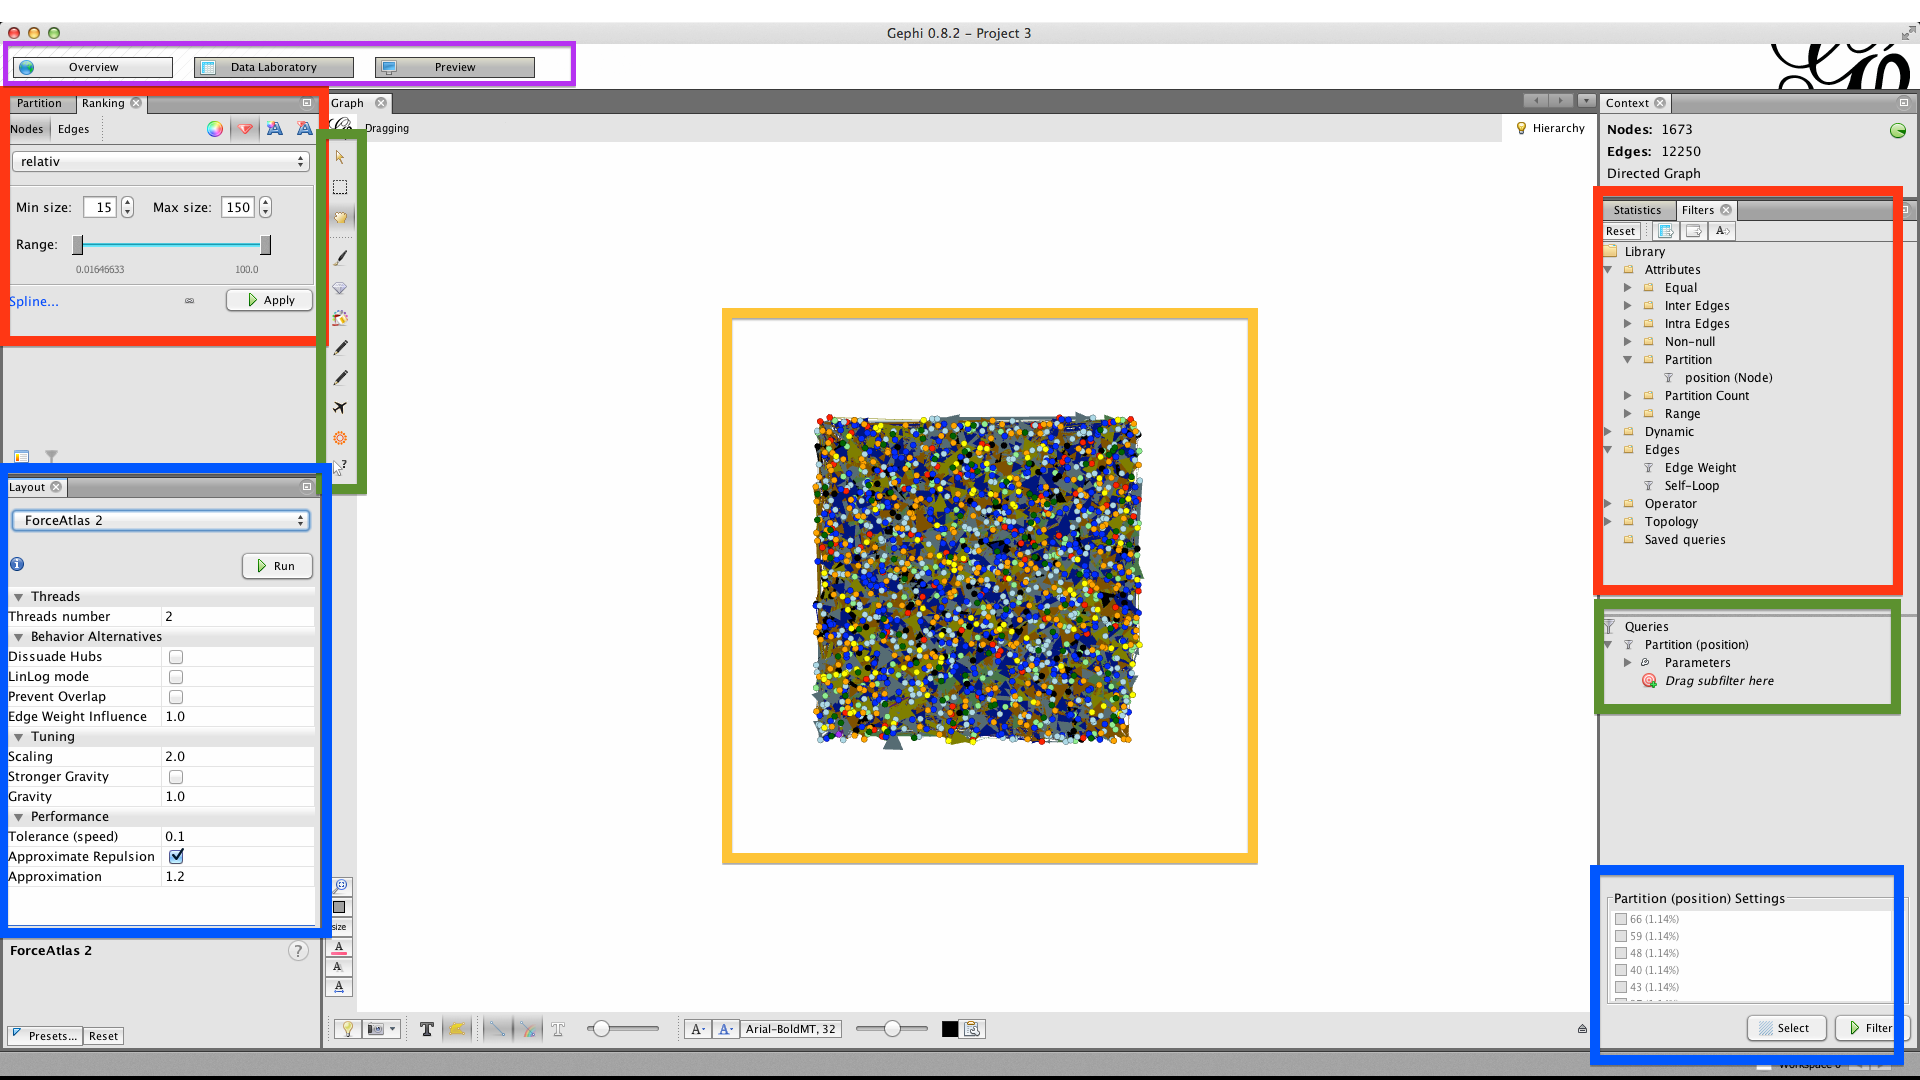
\includegraphics[scale=0.25]{workspace.png}
    \caption[workspace]{Der Workspace in Gephi}
    \label{workspace}
\end{figure}


\subsection*{Ergebnisse und Interpretation mit Gephi}
Um Ergebnisse und Erkenntnisse aus den erstellten Grafiken zu ziehen und zu gewinnen, kann man durch das scrollen in den Graphen hineinzoomen und durch Halten des Rechtsklickes durch den Graphen durch zu ziehen navigieren. Wenn man dann eine aussagekräfige Position im Graphen gefunden hat, wird durch das drüber schweben der Maus über einen Knoten die Verbindung von und zu diesem Knotenpunkt ersichtlich. In der Grafik unten ist dieser Fall beispielsweise an der Position 7 dargestellt. In diesem Fall wurde der Success Knoten ausgewählt und die relativen Ausgänge als Gewichtung. Hier sieht man, aber auch dass es Sinn macht weiterhin Filter zu benutzen um bedeutendere Ergebnisse zu erzielen.


\begin{figure}[H]
    \centering
    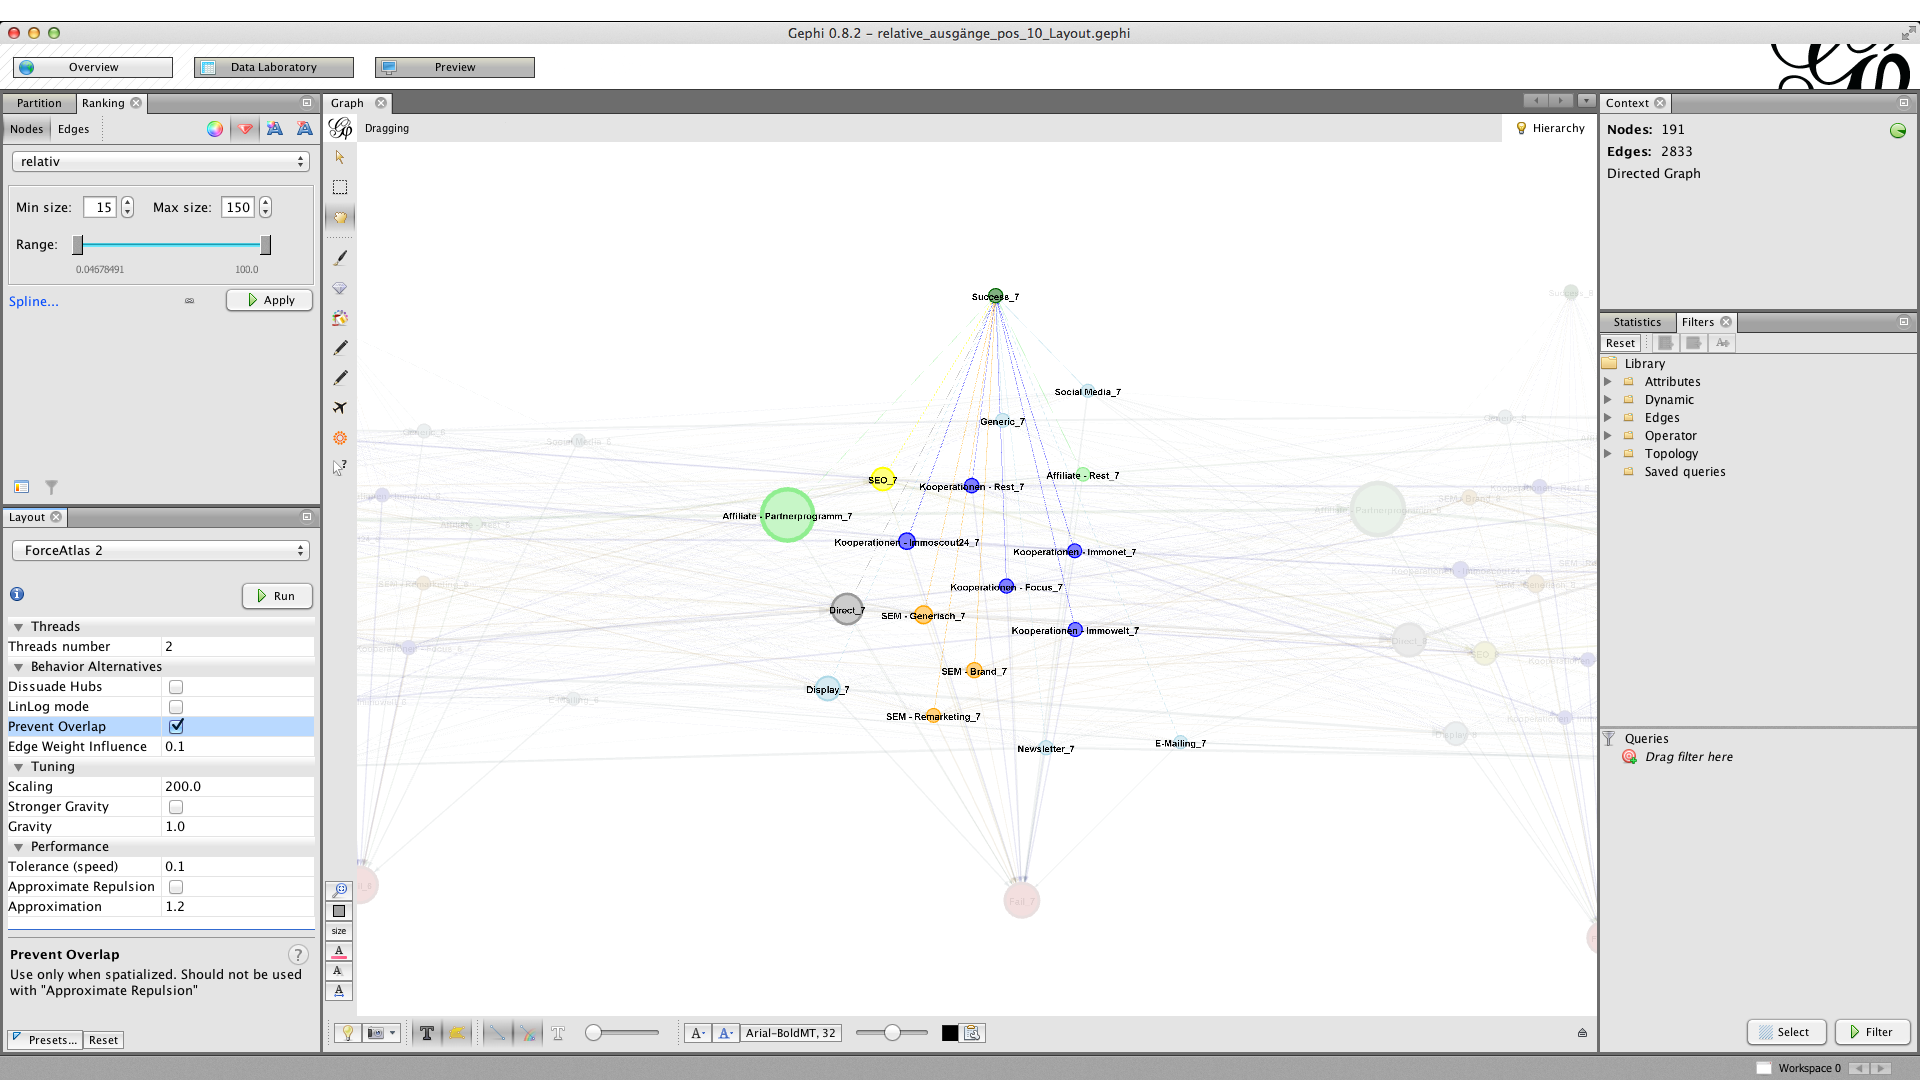
\includegraphics[scale=0.25]{ergebnis_gephi.png}
    \caption[ergebnis]{Ergebnisse in Gephi}
    \label{ergebnis}
\end{figure}


\subsection*{Export in Gephi}
Wenn man dann einen Graphen soweit bearbeitet hat und das Gesamtergebnis exportieren will, kann man das in dem Reiter Preview machen. Nützliche Einstellungen hier sind zum Beispiel im lila Feld \textit{Rescale Weight}, damit die Kanten nicht zu dick sind und das ausstellen von \textit{Curved}, weil diese Funktion zwar den Graphen schön aussehen lässt, aber unübersichtlicher macht. In der grünen Box muss man nach jeder Einstellung den \textit{Refresh} Button klicken und kann zusätzlich den Graphn als SVG-,PDF- oder PNG-Format abspeichern.

\begin{figure}[H]
    \centering
    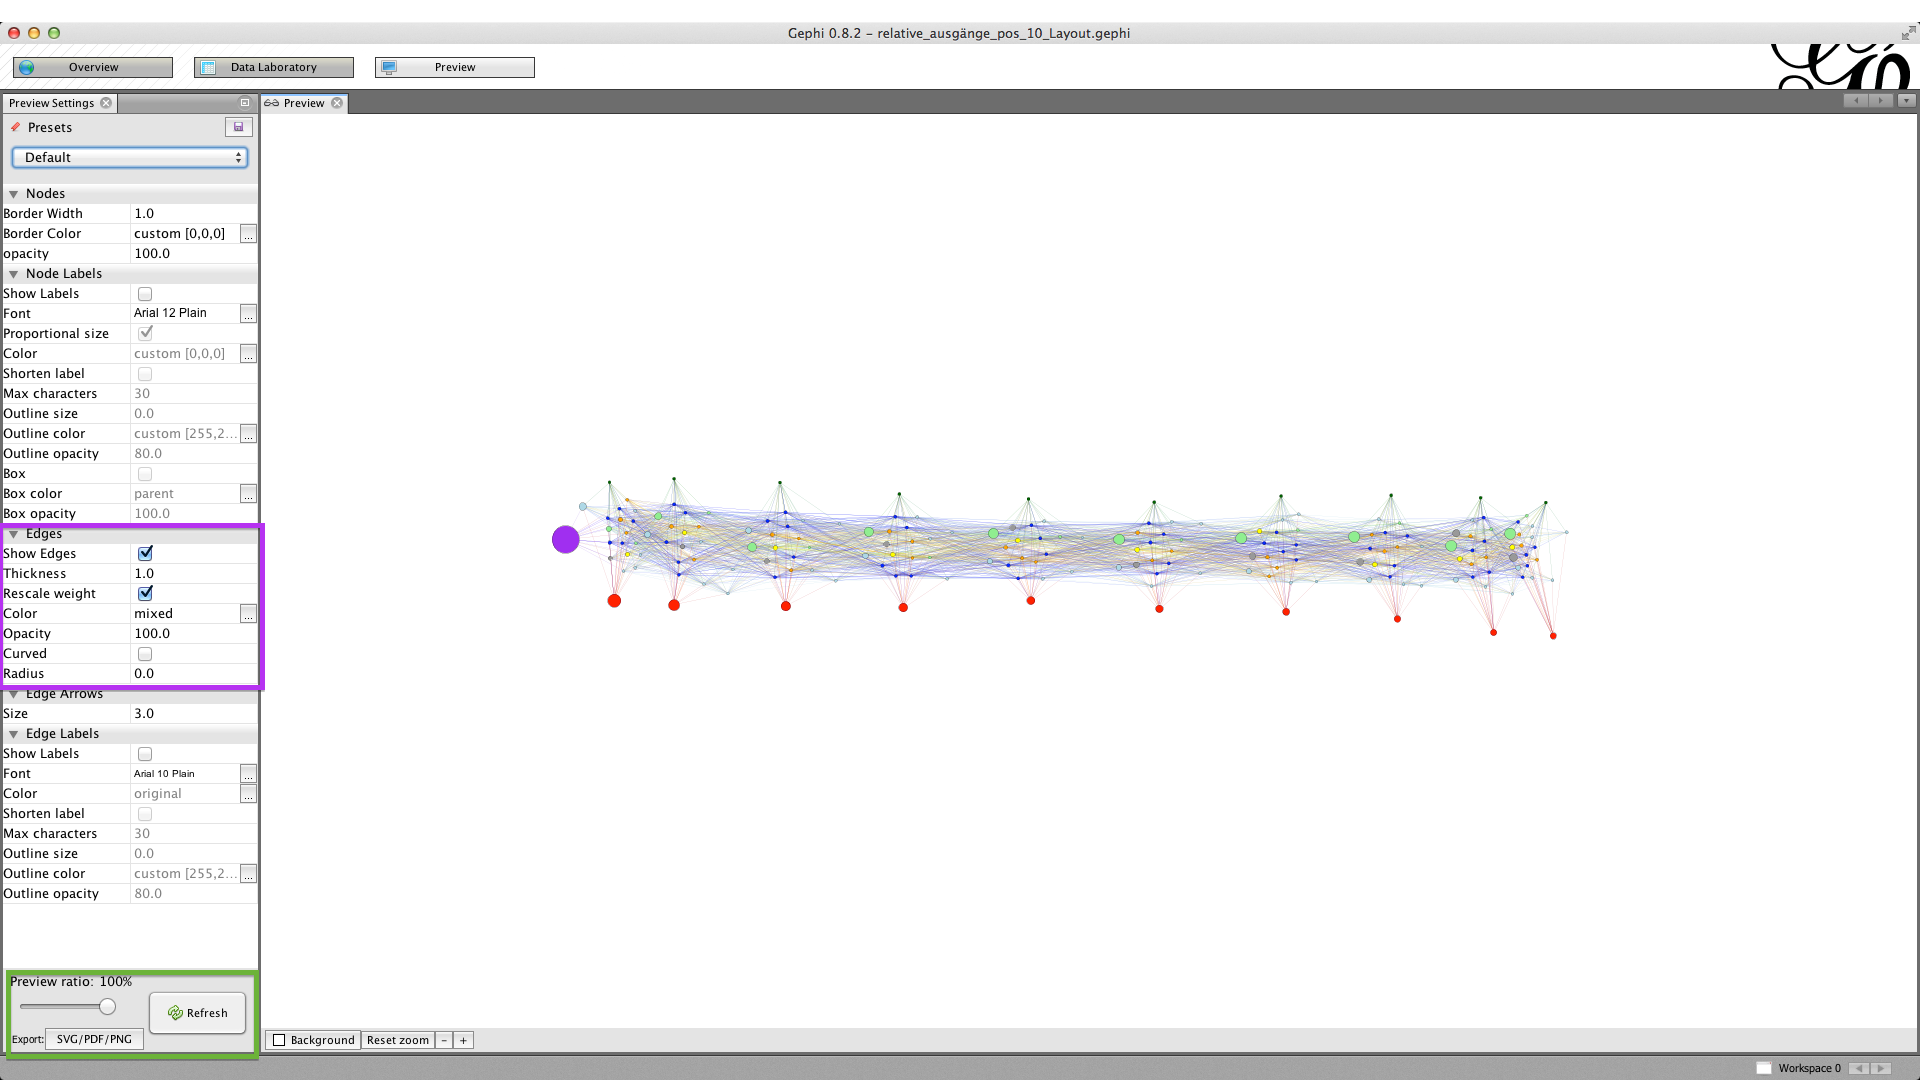
\includegraphics[scale=0.25]{Preview.png}
    \caption[export]{Der Export in Gephi}
    \label{export}
\end{figure}



